% =====================================================================
% DBA - Proyecto final - Entrega 4
% Flujo reproducible de conteo y área de techos por municipio PDET
% =====================================================================
\documentclass[11pt,a4paper]{article}
% =====================================================================
% Preámbulo compartido - DBA Proyecto final
% =====================================================================
\usepackage[utf8]{inputenc}
\usepackage[T1]{fontenc}
\IfFileExists{lmodern.sty}{\usepackage{lmodern}}{}
\usepackage[spanish,es-noshorthands,es-tabla]{babel}
\usepackage[margin=2.5cm]{geometry}
\usepackage{amsmath,amssymb}
\usepackage{booktabs,tabularx,array}
\usepackage{enumitem}
\usepackage[dvipsnames,table]{xcolor}
\usepackage{graphicx}
\usepackage{tikz}
\usetikzlibrary{calc,positioning}
\usepackage{listings}
\usepackage{caption}
\usepackage{float}
\usepackage[hidelinks]{hyperref}
\usepackage{xurl}

% --- Colores --------------------------------------------------------
\definecolor{acento}{HTML}{2F6FDB}
\definecolor{gris}{HTML}{6B6B6B}
\hypersetup{colorlinks=true, linkcolor=acento, urlcolor=acento, citecolor=acento}

% --- Tablas ---------------------------------------------------------
\newcolumntype{L}{>{\raggedright\arraybackslash}X}
\renewcommand{\arraystretch}{1.25}

% --- Listas ---------------------------------------------------------
\setlist{itemsep=2pt, topsep=4pt}

% --- Código (JSON / mongosh) ----------------------------------------
\lstdefinestyle{codigo}{
  basicstyle=\ttfamily\footnotesize,
  breaklines=true,
  columns=fullflexible,
  keepspaces=true,
  frame=single,
  framerule=0.3pt,
  rulecolor=\color{gray!50},
  backgroundcolor=\color{gray!6},
  xleftmargin=4pt, xrightmargin=4pt,
  showstringspaces=false,
  literate={á}{{\'a}}1 {é}{{\'e}}1 {í}{{\'i}}1 {ó}{{\'o}}1 {ú}{{\'u}}1
           {Á}{{\'A}}1 {É}{{\'E}}1 {Í}{{\'I}}1 {Ó}{{\'O}}1 {Ú}{{\'U}}1
           {ñ}{{\~n}}1 {Ñ}{{\~N}}1
}
\lstset{style=codigo}

% --- Atajos ---------------------------------------------------------
\newcommand{\campo}[1]{\texttt{#1}}
\newcommand{\pendiente}[1]{\textcolor{gris}{\textit{[Pendiente -- #1]}}}
% Ruta de archivo larga: igual que \campo pero se puede partir en / y _
% (xurl ya amplía los puntos de corte de \url para que esto funcione).
\newcommand{\ruta}[1]{\begingroup\urlstyle{tt}\url{#1}\endgroup}


% Figura opcional: si img/<nombre>.png todavía no existe, el documento compila
% igual y deja un [Pendiente] visible para que no se olvide.
\newcommand{\figopcional}[3]{%
  \begin{figure}[H]
    \centering
    \IfFileExists{img/#1.png}%
      {\includegraphics[width=\textwidth,height=0.42\textheight,keepaspectratio]{img/#1.png}}%
      {\pendiente{captura \texttt{\detokenize{#1}.png}}}
    \caption{#2}
    \label{#3}
  \end{figure}}

\begin{document}

% ------------------------------- Portada -----------------------------
\begin{titlepage}
  \centering
  {\large Pontificia Universidad Javeriana\par}
  {\large Departamento de Ingeniería de Sistemas\par}
  \vspace{0.8cm}
  {\large Administración de Bases de Datos (DBA) -- 2026-30\par}
  \vspace{2.5cm}
  {\Huge\bfseries Proyecto final\par}
  \vspace{1cm}
  {\LARGE Entrega 4: Flujo reproducible de conteo\\ y área de techos por municipio PDET\par}
  \vspace{1cm}
  {\large Potencial solar en techos de los municipios PDET\par}
  \vspace{3cm}
  {\large
    Maria Camila Beltran \\
    \vspace{0.5cm}
    Jorge Fortich \\
    \vspace{0.5cm}
    Jose Eduardo Valeriano \\
    \vspace{0.5cm}
    Samuel Osorio Rodríguez\par}
  \vspace{3cm}
  {\large Profesor: Andrés Oswaldo Calderón Romero, Ph.D.\par}
  \vspace{3cm}
  {\large Noviembre 23 de 2026\par}
\end{titlepage}

\tableofcontents
\newpage

% =====================================================================
% 1. Contexto y cifras principales (Maria Camila)
% =====================================================================
\section{Contexto y cifras principales}
\label{sec:contexto}

Esta entrega corresponde a la \textbf{semana 4} del plan de implementación:
asignar cada edificio a su municipio PDET, calcular el número de edificios y el
área total de techos por municipio con las dos fuentes, y presentar los
resultados en tablas, mapas y un ranking de municipios candidatos para los
pilotos de granjas solares de la UPME. Todo el cálculo corre dentro de MongoDB
y se reproduce con un solo comando, \campo{make all}
(sección~\ref{sec:reproduccion}).

La tabla~\ref{tab:resumen4} reúne las cifras de las cuatro semanas. Las de esta
entrega salen de la misma corrida que los CSV versionados en
\ruta{data/processed/}.

\begin{table}[H]
  \centering\small
  \caption{Cifras principales del proyecto (escenario base: Google con confianza $\geq 0{,}65$).}
  \label{tab:resumen4}
  \begin{tabularx}{\textwidth}{@{}L r r@{}}
    \toprule
    & \textbf{Google} & \textbf{Microsoft} \\
    \midrule
    Municipios PDET cargados (MGN 2025) & \multicolumn{2}{c}{170 (16 subregiones, 19 departamentos)} \\
    Área total de los municipios PDET & \multicolumn{2}{c}{389\,182\,km\textsuperscript{2}} \\
    Edificios en PDET (en la colección) & 2\,694\,786 & 1\,761\,048 \\
    Edificios asignados a un municipio & 2\,694\,785 & 1\,761\,048 \\
    Municipios sin ningún edificio & 5 & 0 \\
    Área total de techos & 222,17\,km\textsuperscript{2} & 221,13\,km\textsuperscript{2} \\
    Área media por edificio & 82,4\,m\textsuperscript{2} & 125,6\,m\textsuperscript{2} \\
    Documentos en \campo{resultados} & 510 (3 umbrales) & 170 \\
    \bottomrule
  \end{tabularx}
\end{table}

% =====================================================================
% 2. Plan de implementación y estado (Maria Camila)
% =====================================================================
\section{Plan de implementación y estado}
\label{sec:plan}

\begin{table}[H]
  \centering\small
  \caption{Plan de implementación y estado.}
  \label{tab:plan}
  \begin{tabularx}{\textwidth}{@{}l L L l@{}}
    \toprule
    Semana & Fase & Resultado principal & Estado \\
    \midrule
    1 & Esquema y plan & Diseño NoSQL, diagrama E-R, diccionario de datos & Hecha \\
    2 & Límites PDET & 170 municipios cargados, validados e indexados & Hecha \\
    3 & Huellas de edificios & Google y Microsoft descargados, limpios, cargados e
        indexados; EDA breve & Hecha \\
    4 & Análisis & Asignación por centroide, agregación en \campo{resultados},
        sensibilidad, mapas y ranking & \textbf{Esta entrega} \\
    Final & Informe técnico & Documento autocontenido para la UPME (26 de noviembre) & Siguiente \\
    \bottomrule
  \end{tabularx}
\end{table}

\textbf{Organización del equipo.} Un archivo por tarea en
\campo{src/analisis/}, una rama y un \emph{pull request} por persona, con
revisión de alguien de otro frente antes del merge a \campo{main}. Reparto de
esta semana: asignación, evidencia y validación (Jorge); estilo de figuras y
correcciones al EDA (Jose Eduardo); agregación, sensibilidad y exportación
(Samuel); mapas, ranking, \campo{run.py} e integración del informe (Maria
Camila).

% =====================================================================
% 3. Resumen de las semanas 2 y 3 (criterios 1 a 3) (Maria Camila)
% =====================================================================
\section{Resumen de adquisición, integridad y carga}
\label{sec:resumen-previo}

La rúbrica de esta semana vuelve a calificar lo construido en las entregas 2 y
3. Aquí se resume en una página; el detalle, con capturas, está en esas
entregas.

\begin{table}[H]
  \centering\small
  \caption{Adquisición y verificación de las tres fuentes.}
  \label{tab:adquisicion}
  \begin{tabularx}{\textwidth}{@{}p{2.6cm} L L L@{}}
    \toprule
    & \textbf{MGN 2025 (DANE)} & \textbf{Google Open Buildings v3} & \textbf{Microsoft Building Footprints} \\
    \midrule
    Descarga & ZIP nivel municipio (68\,MB) & 8 celdas S2 (3,11\,GB) & 125 \emph{quadkeys} (373,4\,MB) \\
    Trazabilidad & SHA-256 en \campo{fuentes} & SHA-256 por archivo en \campo{fuentes} & SHA-256 global en \campo{fuentes} \\
    Filtro a PDET & Cruce por código DANE (5 dígitos) con \campo{MunicipiosPDET.xlsx} & Prefiltro con DuckDB por centroide & Prefiltro con DuckDB por centroide \\
    Verificación & 170 de 170 cruzaron; 16 subregiones y 19 departamentos & 16\,512\,141 leídos $\rightarrow$ 2\,694\,786 en PDET & 4\,595\,615 leídos $\rightarrow$ 1\,761\,048 en PDET \\
    \bottomrule
  \end{tabularx}
\end{table}

\textbf{Integridad y formato.} Las cuatro colecciones con datos
(\campo{municipios}, \campo{edificios\_google}, \campo{edificios\_microsoft} y
\campo{resultados}) tienen validación \campo{\$jsonSchema} estricta. Las
geometrías se revisaron con \campo{is\_valid} de GEOS y se repararon con
\campo{make\_valid}: las 170 de los municipios venían válidas, Google no tuvo
ninguna inválida y Microsoft tuvo 28. Además, 29 polígonos de Microsoft eran
válidos para GEOS pero MongoDB los rechazaba por su validación esférica (S2);
se repararon en la carga. Todo se guarda en WGS84 (\campo{[lon, lat]}, lo que
exige el índice \campo{2dsphere}) y las áreas se calculan en EPSG:9377 (metros).
El índice único sobre \campo{geom\_hash} confirmó que no hay duplicados.

\textbf{Eficiencia de carga.} Los Parquet se leen por lotes de 5\,000 filas y
se insertan con \campo{insert\_many(ordered=False)}; los índices de
\campo{centroide}, \campo{cod\_mpio} y \campo{geom\_hash} se crean después de
cargar, porque mantenerlos durante la inserción es más lento. Google se cargó
en 56,6\,s (47\,621\,docs/s) y Microsoft en 37,7\,s (46\,753\,docs/s). En esta
semana se sumó el costo de la asignación: 269,9\,s para Google y 182,1\,s para
Microsoft usando el índice \campo{centroide\_2dsphere}; sin él, una sola
consulta \campo{\$geoWithin} recorre la colección completa y tarda unas 10
veces más (sección~\ref{sec:explain4}).

\textbf{Análisis exploratorio.}\label{sec:eda} El EDA de la Entrega~3 mostró
que las dos fuentes cubren casi la misma superficie, que Google reparte esa
superficie en huellas más pequeñas y que cinco municipios del Chocó y del
Atrato antioqueño no tienen ningún edificio en Google (mapa de control de la
Entrega~3). Las cuatro figuras del EDA se rehicieron con
\campo{figuras\_eda.py} y el estilo común \campo{estilo.py}; la comparación
antes y después está en la sección de correcciones de la Entrega~3.

% =====================================================================
% 4. Asignación por centroide y validación (Jorge)
% =====================================================================
\InputIfFileExists{seccion_asignacion.tex}{}{%
  \section{Asignación por centroide y validación}\pendiente{sección de Jorge (seccion\_asignacion.tex)}}
\label{sec:explain4}

% =====================================================================
% 6. Agregación y sensibilidad (Samuel)
% =====================================================================
\InputIfFileExists{seccion_agregacion.tex}{}{%
  \section{Agregación y sensibilidad}\pendiente{sección de Samuel (seccion\_agregacion.tex)}}

% =====================================================================
% 7. Lectura de los resultados (Jose Eduardo)
% =====================================================================
\InputIfFileExists{seccion_resultados.tex}{}{%
  \section{Lectura de los resultados}\pendiente{sección de Jose Eduardo (seccion\_resultados.tex)}}

% =====================================================================
% 8. Mapas de resultados (Maria Camila)
% =====================================================================
\section{Mapas de resultados por municipio}
\label{sec:resultados}

Esta sección cubre \campo{mapas.py}, en \campo{src/analisis/}. Los mapas no
necesitan la base de datos: leen los dos archivos versionados en el
repositorio, \ruta{data/processed/municipios_pdet.geojson} (límites) y
\ruta{data/processed/resultados_municipio.csv} (lo que exporta
\campo{exportar.py}), así que cualquiera puede rehacerlos con
\campo{python -m src.analisis.run --solo-figuras}. Todos usan el escenario base
y las reglas de figuras del equipo: textos en español, unidades en la leyenda,
contorno de las 16 subregiones y municipios sin dato en gris con trama. Las
áreas se expresan en hectáreas (1\,ha $=$ 10\,000\,m\textsuperscript{2}),
que se leen mejor que los km\textsuperscript{2} a escala de municipio. La
tabla por subregión está en la sección de agregación
(tabla~\ref{tab:subregion}).

\subsection{Área de techos por fuente}

La figura~\ref{fig:mapa-fuentes} pone las dos fuentes lado a lado con las
\emph{mismas} cinco clases. Las clases son los quintiles del área por
municipio calculados sobre las dos fuentes juntas (340 valores, sin ceros):
si cada mapa tuviera sus propios cortes, el mismo color significaría cosas
distintas y no se podrían comparar. Se usa una escala secuencial de un solo
tono (verde) para que no se confunda con el azul y el naranja que identifican
a cada fuente en el resto del informe.

\begin{figure}[H]
  \centering
  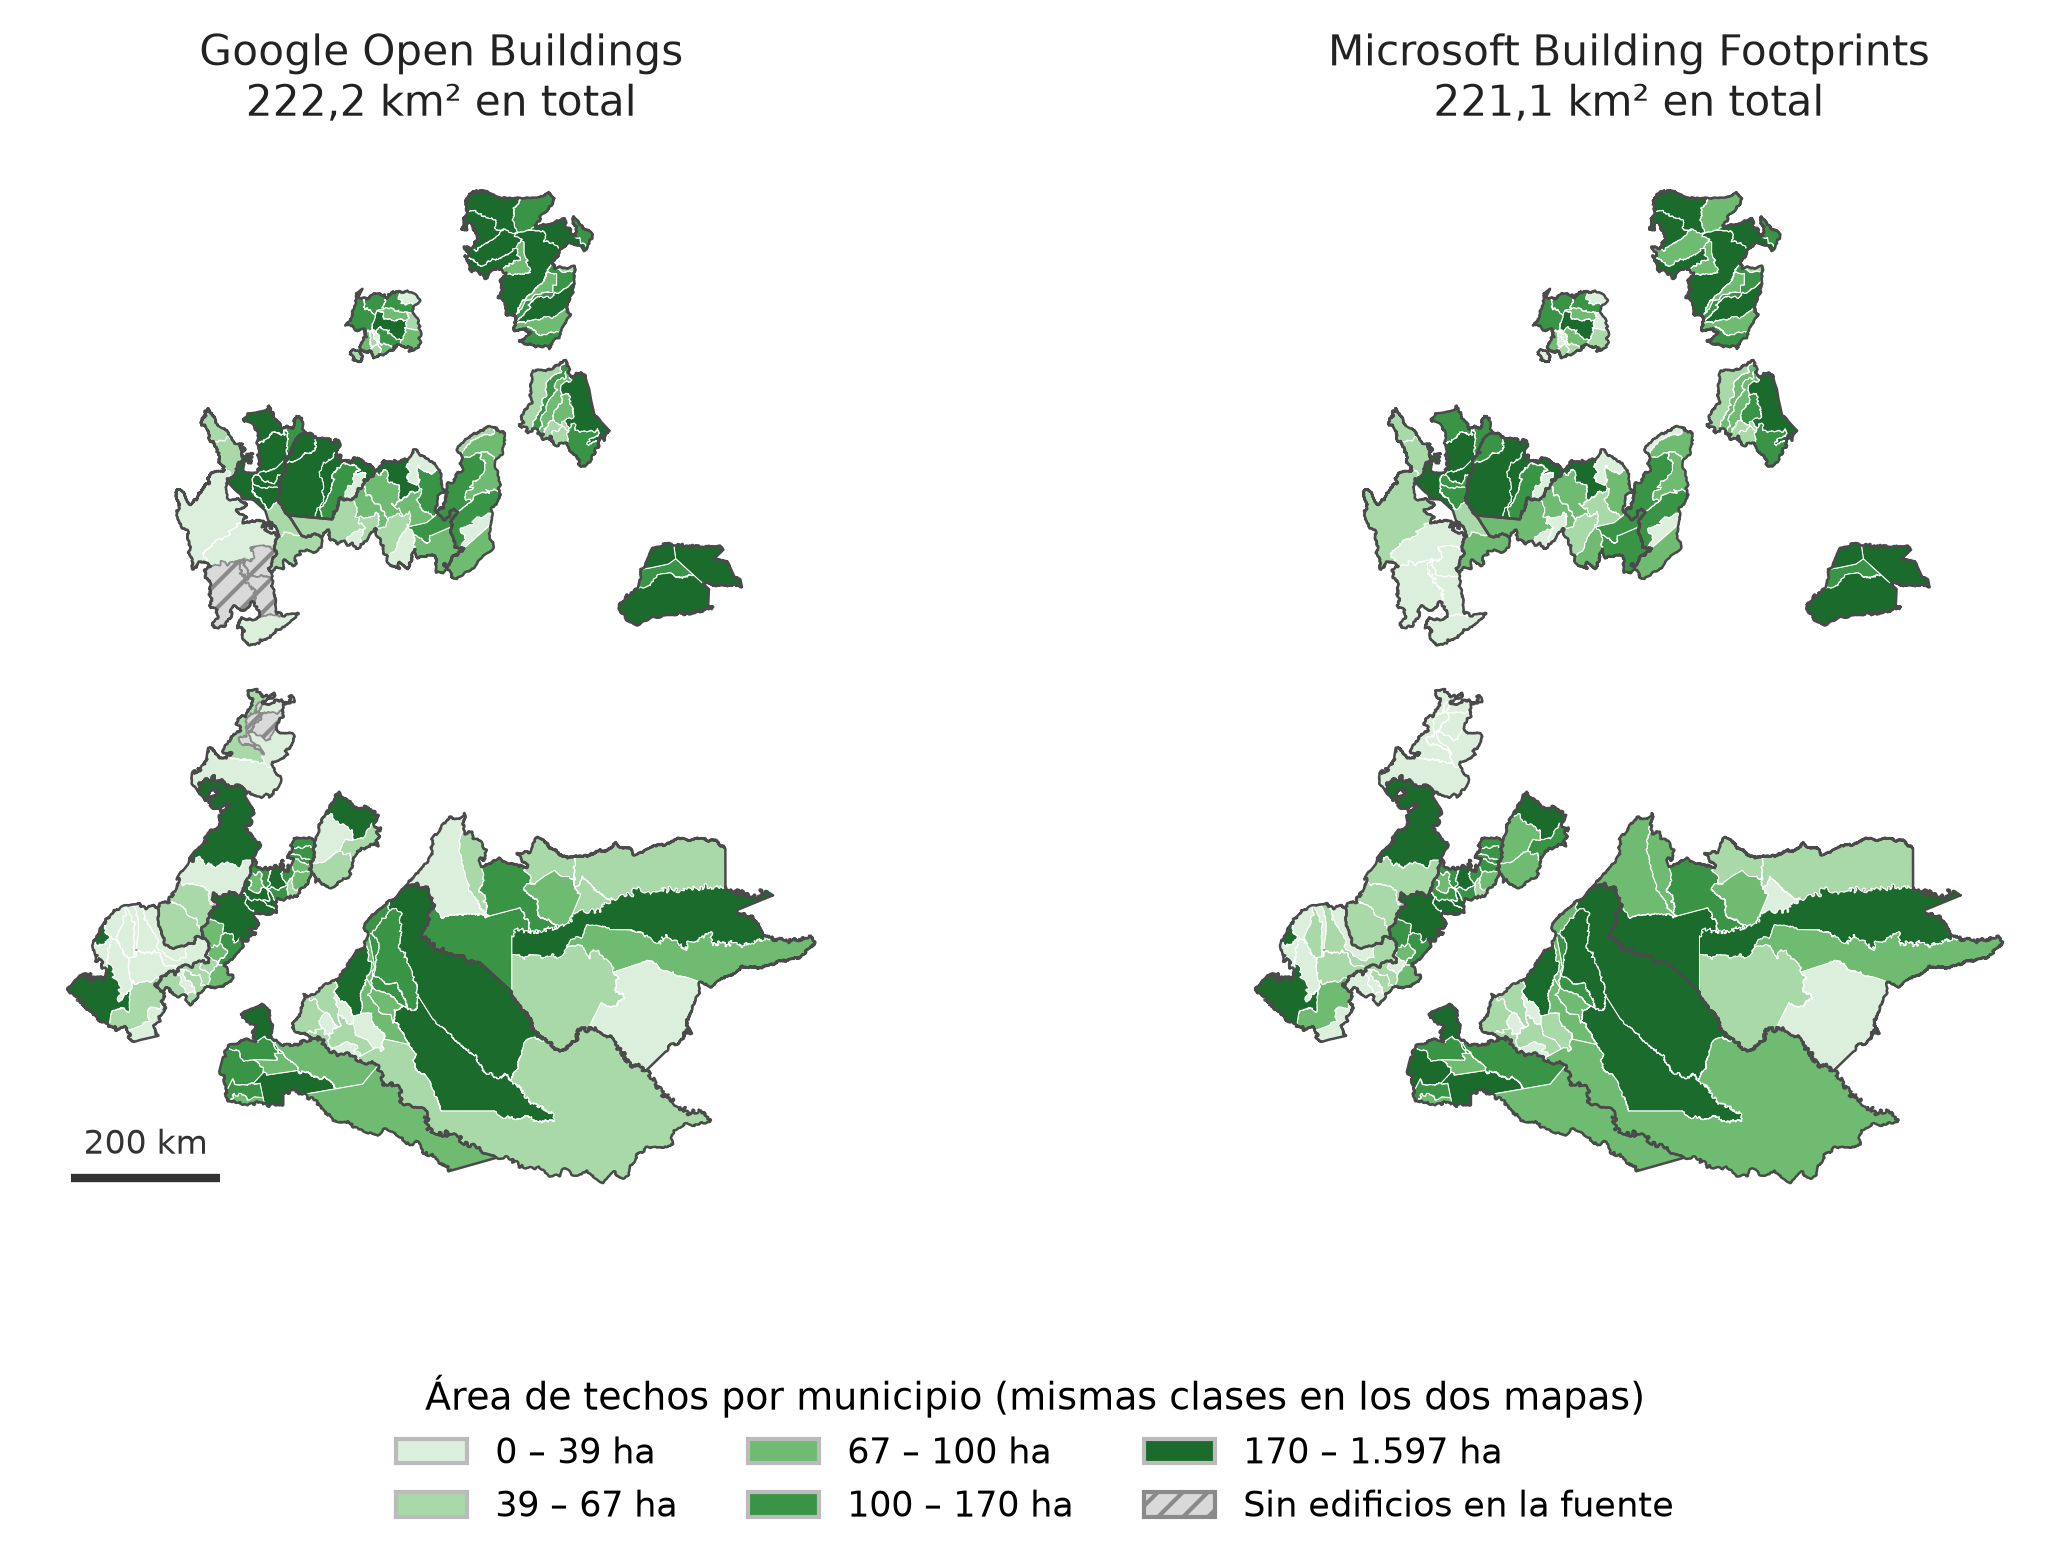
\includegraphics[width=\textwidth]{img/mapa_area_fuentes.png}
  \caption{Área de techos por municipio PDET, Google (izquierda) y Microsoft
  (derecha), con las mismas clases. En gris con trama, los 5 municipios sin
  edificios en Google.}
  \label{fig:mapa-fuentes}
\end{figure}

Los dos mapas cuentan la misma historia en casi todo el territorio. El área se
concentra en los municipios con cabeceras urbanas grandes (Santa Marta y
Valledupar superan las 1\,300\,ha con las dos fuentes) y en la Sierra Nevada -
Perijá, Urabá, el norte del Cauca y el piedemonte caqueteño. Los municipios
extensos de la Amazonía y la Orinoquía, aunque ocupan buena parte del mapa,
tienen poca área de techos. La diferencia visible está en el Chocó y la costa
pacífica nariñense, que son más claros en Google. La correlación entre las dos
fuentes por municipio es alta (Pearson 0,99; Spearman 0,94 sobre los 170
municipios), como también muestra la dispersión de la
figura~\ref{fig:res-dispersion}.

\subsection{Diferencia entre fuentes}

La figura~\ref{fig:mapa-diferencia} muestra el índice
$D = (A_G - A_M)/(A_G + A_M)$, que va de $-1$ (solo Microsoft tiene edificios)
a $+1$ (solo Google). La escala es divergente y está centrada en 0: naranja
donde Microsoft tiene más área, azul donde la tiene Google y gris donde las dos
coinciden ($|D| \leq 0{,}1$).

\begin{figure}[H]
  \centering
  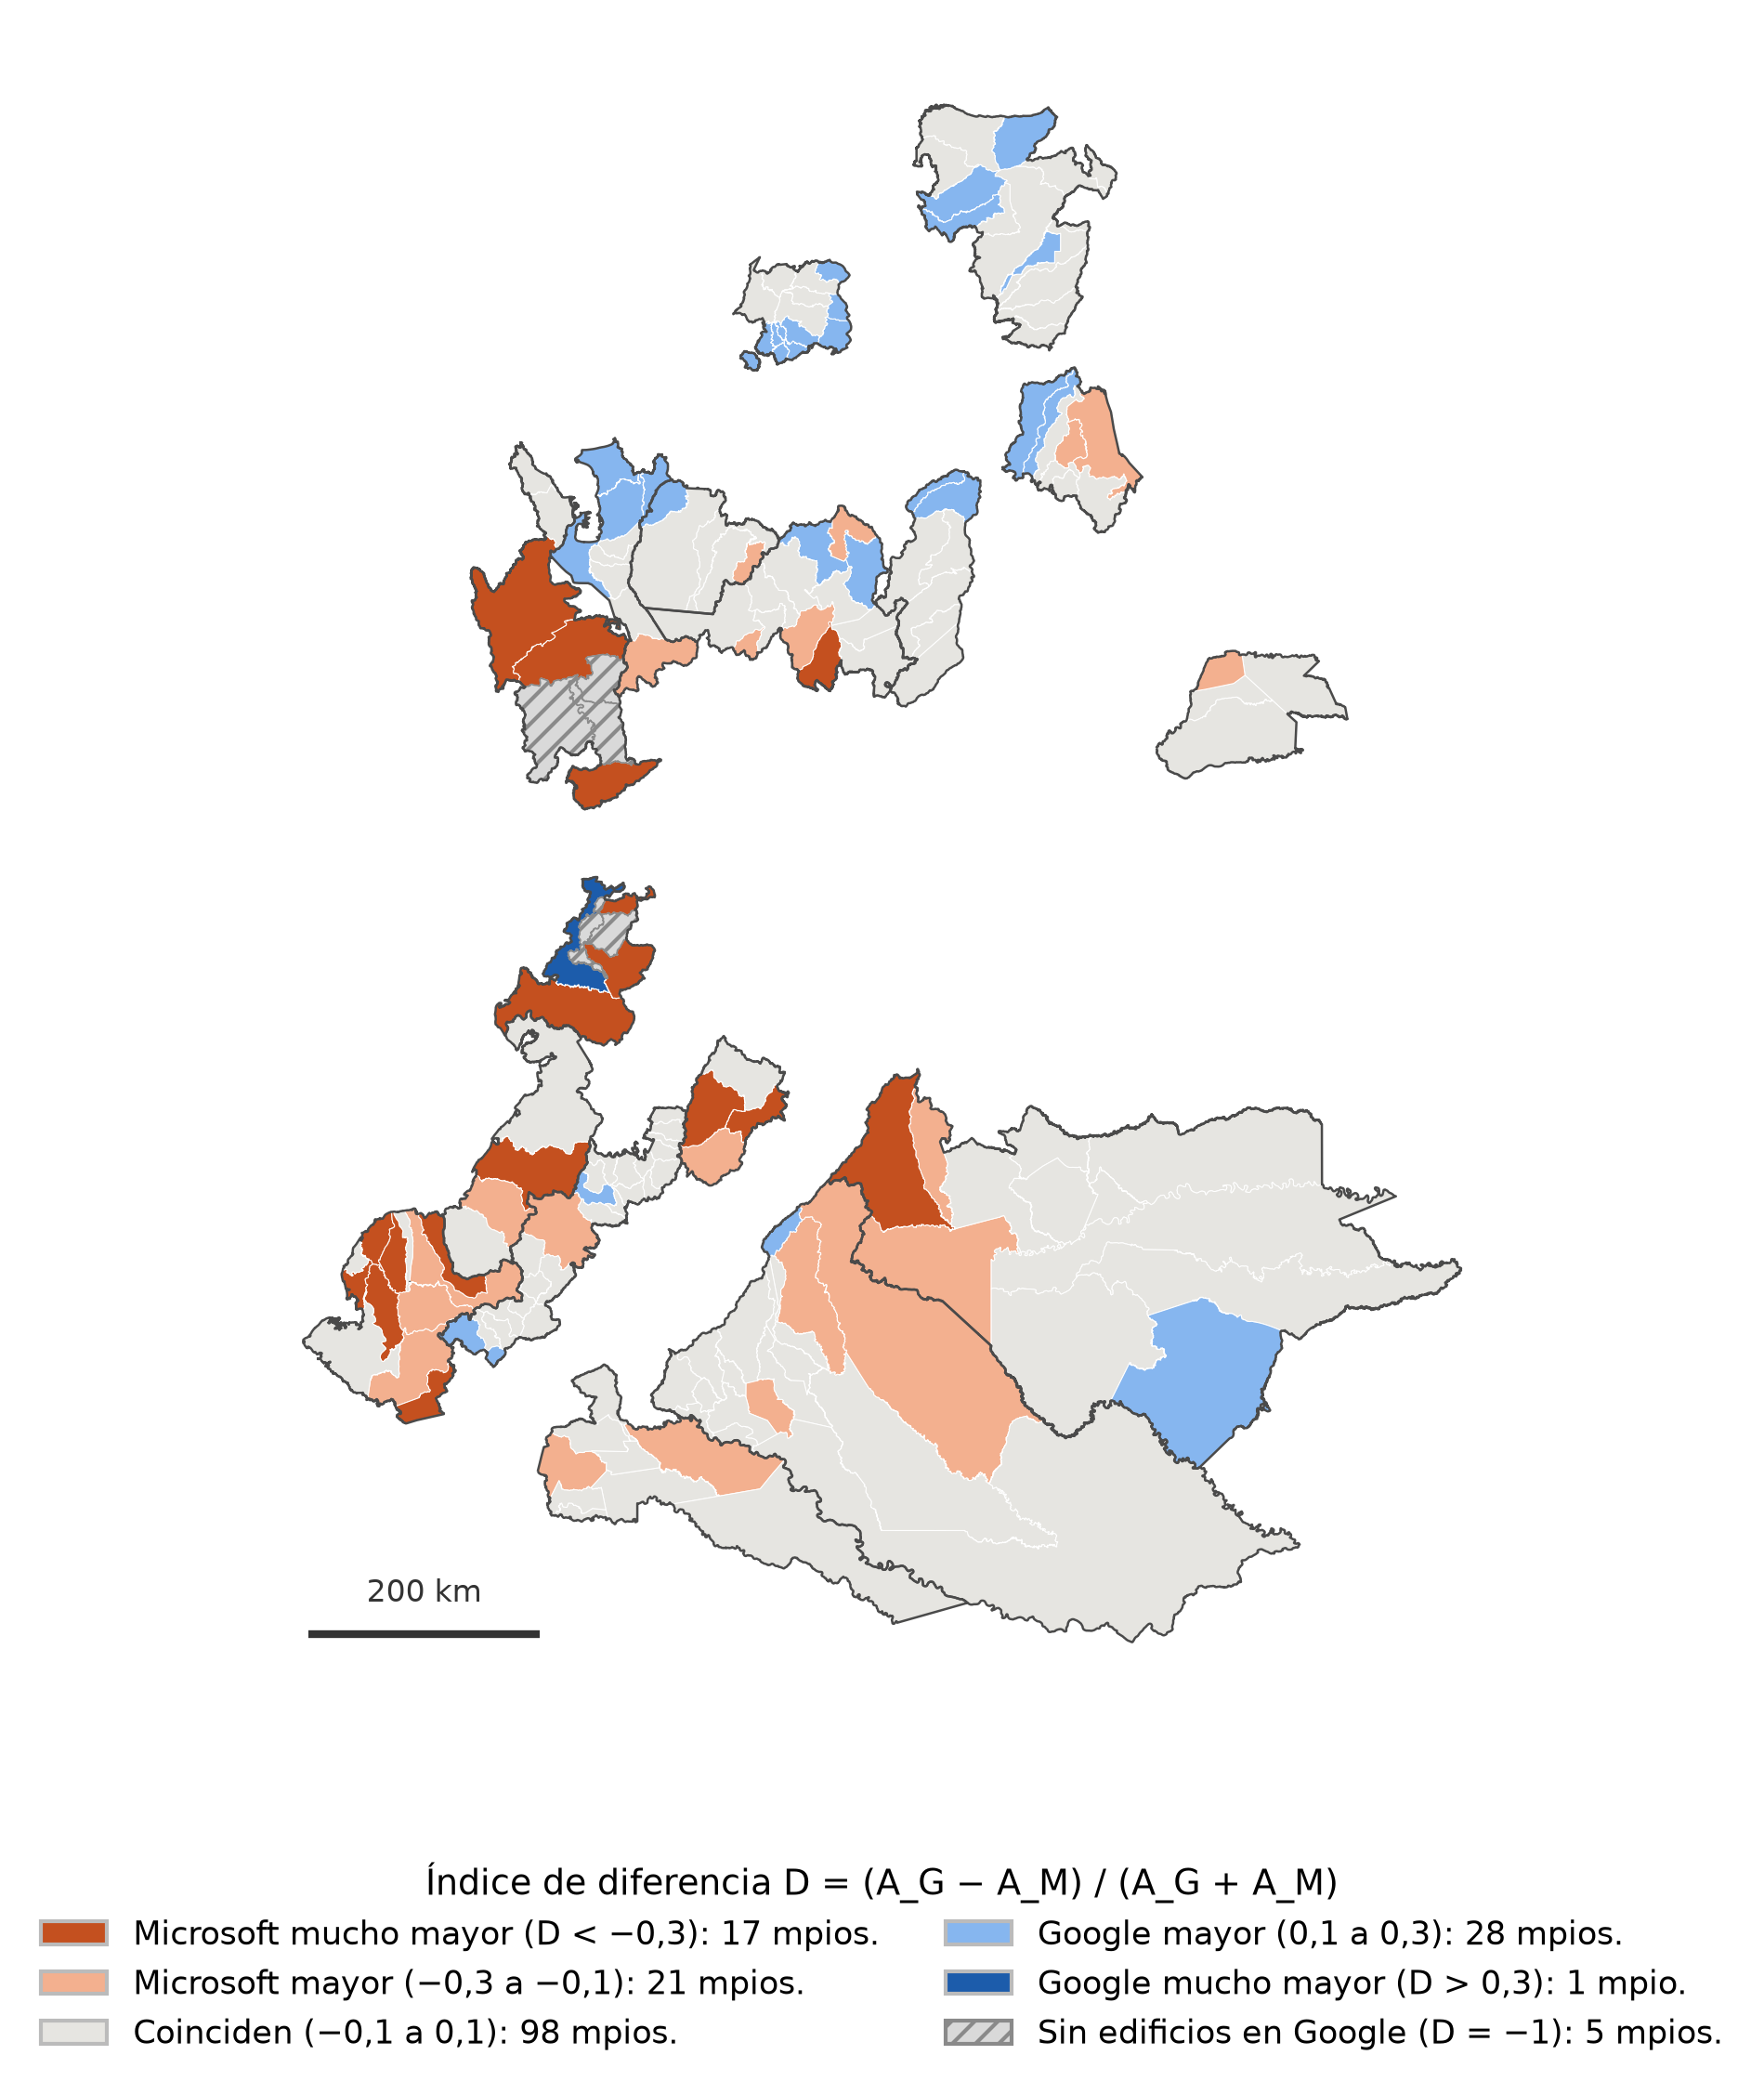
\includegraphics[width=0.92\textwidth]{img/mapa_diferencia.png}
  \caption{Índice de diferencia $D$ entre Google y Microsoft por municipio
  (escenario base).}
  \label{fig:mapa-diferencia}
\end{figure}

En 98 de los 170 municipios las fuentes coinciden dentro de $\pm 10$\,\% y en
otros 49 la diferencia es moderada. Los 23 municipios con desacuerdo fuerte
($|D| > 0{,}3$) no están repartidos al azar: 12 son del Chocó y 6 del
Pacífico y Frontera Nariñense, e incluyen los 5 sin edificios en Google
(Murindó, Vigía del Fuerte, Bojayá, Medio San Juan y Nóvita) y otros como
Sipí, López de Micay, Ricaurte y Carmen del Darién, donde Google detecta menos
del 10\,\% del área que detecta Microsoft. Solo un municipio tiene mucho más
área en Google: Istmina ($D = +0{,}60$).

\subsection{Porcentaje del municipio cubierto por techos}

El área total favorece a los municipios grandes. La
figura~\ref{fig:mapa-pct} normaliza por la superficie del municipio: qué
fracción de su territorio está cubierta por techos (promedio de las dos
fuentes). La mediana es 0,077\,\%; Piendamó - Tunía (1,34\,\%), Santander de
Quilichao (0,78\,\%), Apartadó (0,65\,\%) y Santa Marta (0,64\,\%) encabezan,
y el norte del Cauca aparece como la zona más densa.

\begin{figure}[H]
  \centering
  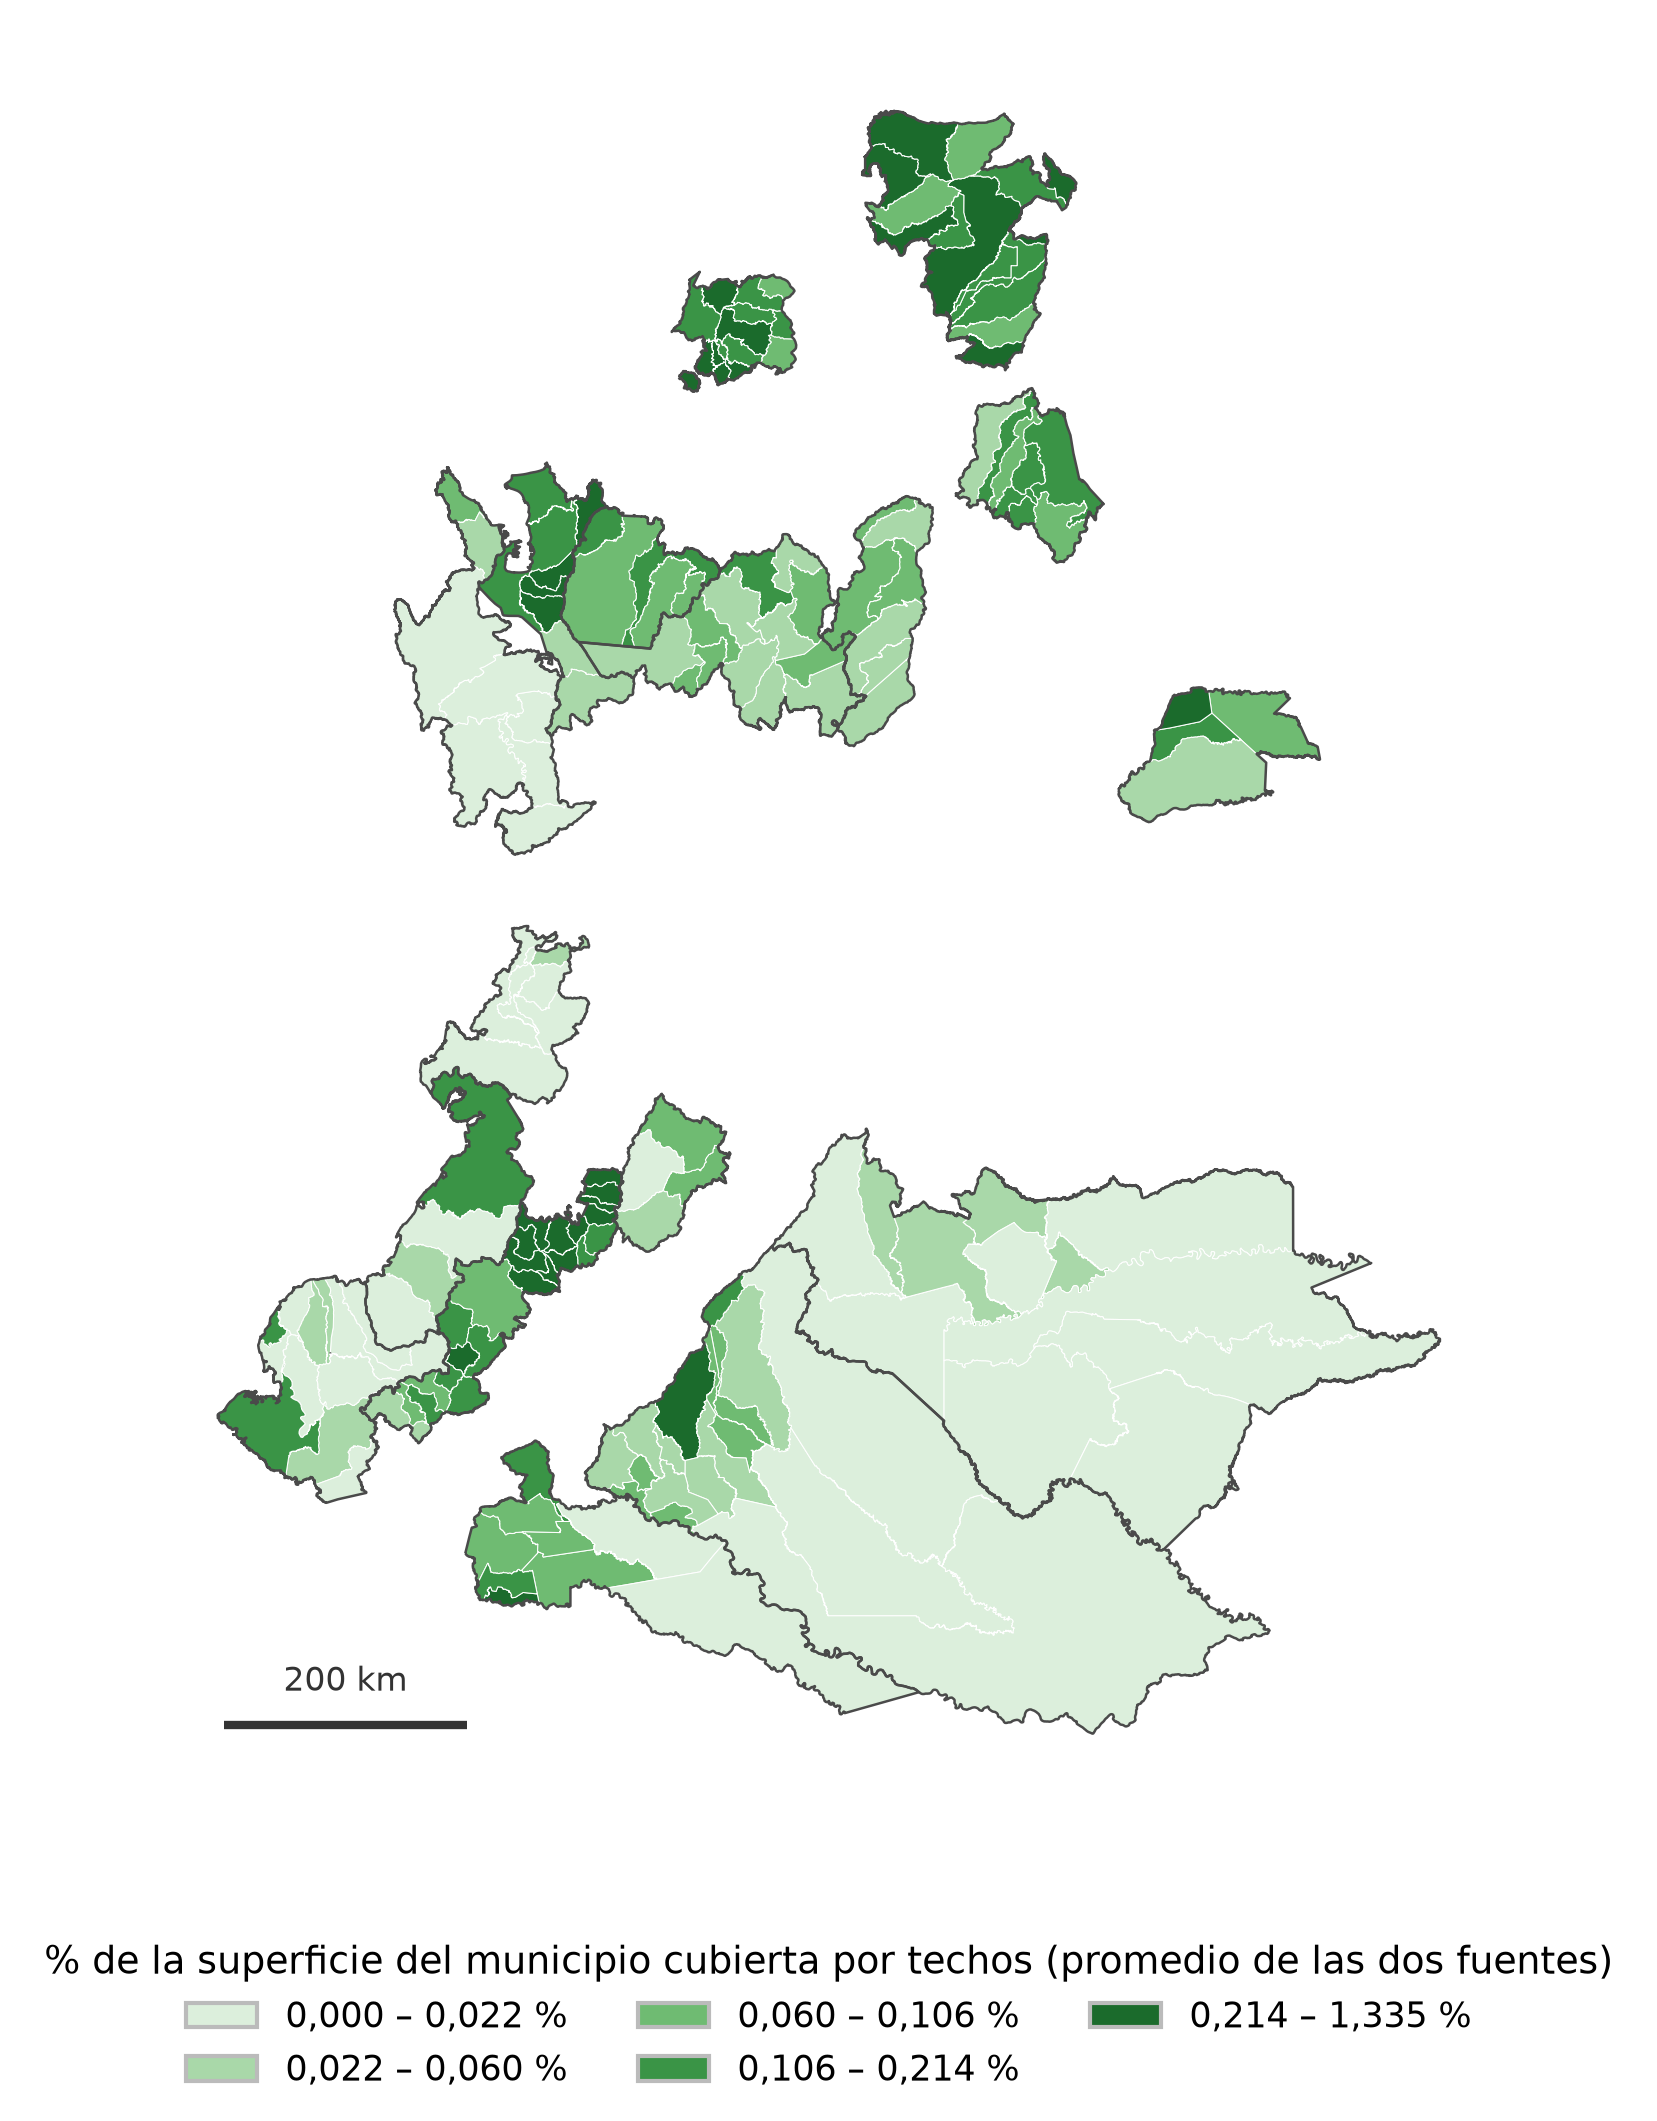
\includegraphics[width=0.85\textwidth]{img/mapa_pct_techos.png}
  \caption{Porcentaje de la superficie municipal cubierta por techos (promedio
  de Google y Microsoft, escenario base). Clases por quintiles.}
  \label{fig:mapa-pct}
\end{figure}

% =====================================================================
% 9. Ranking (Maria Camila)
% =====================================================================
\section{Ranking de municipios candidatos}
\label{sec:ranking}

Esta sección cubre \campo{ranking.py}. El criterio para ordenar es el
\textbf{área conservadora}, $\min(A_G, A_M)$: el área de techos que las dos
fuentes respaldan a la vez. Se descartó ordenar por una sola fuente o por el
promedio, porque así un municipio subiría en el ranking solo porque una de las
dos lo sobreestima. Junto al área se reporta $D$, para marcar los municipios
con fuentes en desacuerdo ($|D| > 0{,}3$), y el porcentaje de techos, que
indica qué tan concentrada está esa área. El ranking completo de los 170
municipios queda en \ruta{data/processed/ranking_municipios.csv}.

\IfFileExists{ranking.tex}{\begin{table}[H]
\centering\scriptsize
\caption{Top 15 de municipios candidatos, ordenados por el área conservadora $\min(A_G, A_M)$ (escenario base: Google con umbral 0,65). Áreas en hectáreas (1\,ha $=$ 10\,000\,m\textsuperscript{2}). $D = (A_G - A_M)/(A_G + A_M)$. \% techos: superficie del municipio cubierta por techos, promedio de las dos fuentes. $^{\dagger}$Fuentes en desacuerdo ($|D| > 0,3$).}
\label{tab:ranking}
\setlength{\tabcolsep}{3.5pt}
\begin{tabularx}{\textwidth}{@{}r>{\raggedright\arraybackslash}p{2.6cm}>{\raggedright\arraybackslash}p{1.7cm}>{\raggedright\arraybackslash}Xrrrrr@{}}
\toprule
 & & & & \multicolumn{3}{c}{\textbf{Área de techos (ha)}} & & \\
\cmidrule(lr){5-7}
\textbf{\#} & \textbf{Municipio} & \textbf{Depto.} & \textbf{Subregión} & \textbf{Google} & \textbf{Microsoft} & \textbf{Conserv.} & $\boldsymbol{D}$ & \textbf{\% techos} \\
\midrule
1 & Santa Marta & Magdalena & Sierra Nevada - Perijá & 1\,597 & 1\,421 & \textbf{1\,421} & $+$0,06 & 0,64 \\
2 & Valledupar & Cesar & Sierra Nevada - Perijá & 1\,531 & 1\,351 & \textbf{1\,351} & $+$0,06 & 0,34 \\
3 & Buenaventura & Valle del Cauca & Pacífico Medio & 766 & 715 & \textbf{715} & $+$0,03 & 0,12 \\
4 & Florencia & Caquetá & Cuenca del Caguán y Piedemonte Caqueteño & 733 & 669 & \textbf{669} & $+$0,05 & 0,28 \\
5 & Turbo & Antioquia & Urabá Antioqueño & 604 & 466 & \textbf{466} & $+$0,13 & 0,18 \\
6 & Santander de Quilichao & Cauca & Alto Patía y Norte del Cauca & 384 & 424 & \textbf{384} & $-$0,05 & 0,78 \\
7 & San Andrés de Tumaco & Nariño & Pacífico y Frontera Nariñense & 379 & 452 & \textbf{379} & $-$0,09 & 0,11 \\
8 & Ciénaga & Magdalena & Sierra Nevada - Perijá & 396 & 347 & \textbf{347} & $+$0,06 & 0,28 \\
9 & Apartadó & Antioquia & Urabá Antioqueño & 360 & 337 & \textbf{337} & $+$0,03 & 0,65 \\
10 & San José del Guaviare & Guaviare & Macarena - Guaviare & 315 & 310 & \textbf{310} & $+$0,01 & 0,02 \\
11 & Tierralta & Córdoba & Sur de Córdoba & 308 & 297 & \textbf{297} & $+$0,02 & 0,06 \\
12 & Arauquita & Arauca & Arauca & 292 & 332 & \textbf{292} & $-$0,06 & 0,10 \\
13 & Tame & Arauca & Arauca & 318 & 276 & \textbf{276} & $+$0,07 & 0,06 \\
14 & Puerto Asís & Putumayo & Putumayo & 266 & 306 & \textbf{266} & $-$0,07 & 0,10 \\
15 & Tibú & Norte de Santander & Catatumbo & 264 & 357 & \textbf{264} & $-$0,15 & 0,12 \\
\bottomrule
\end{tabularx}
\end{table}
}{\pendiente{tabla del ranking (ranking.tex)}}

\begin{figure}[H]
  \centering
  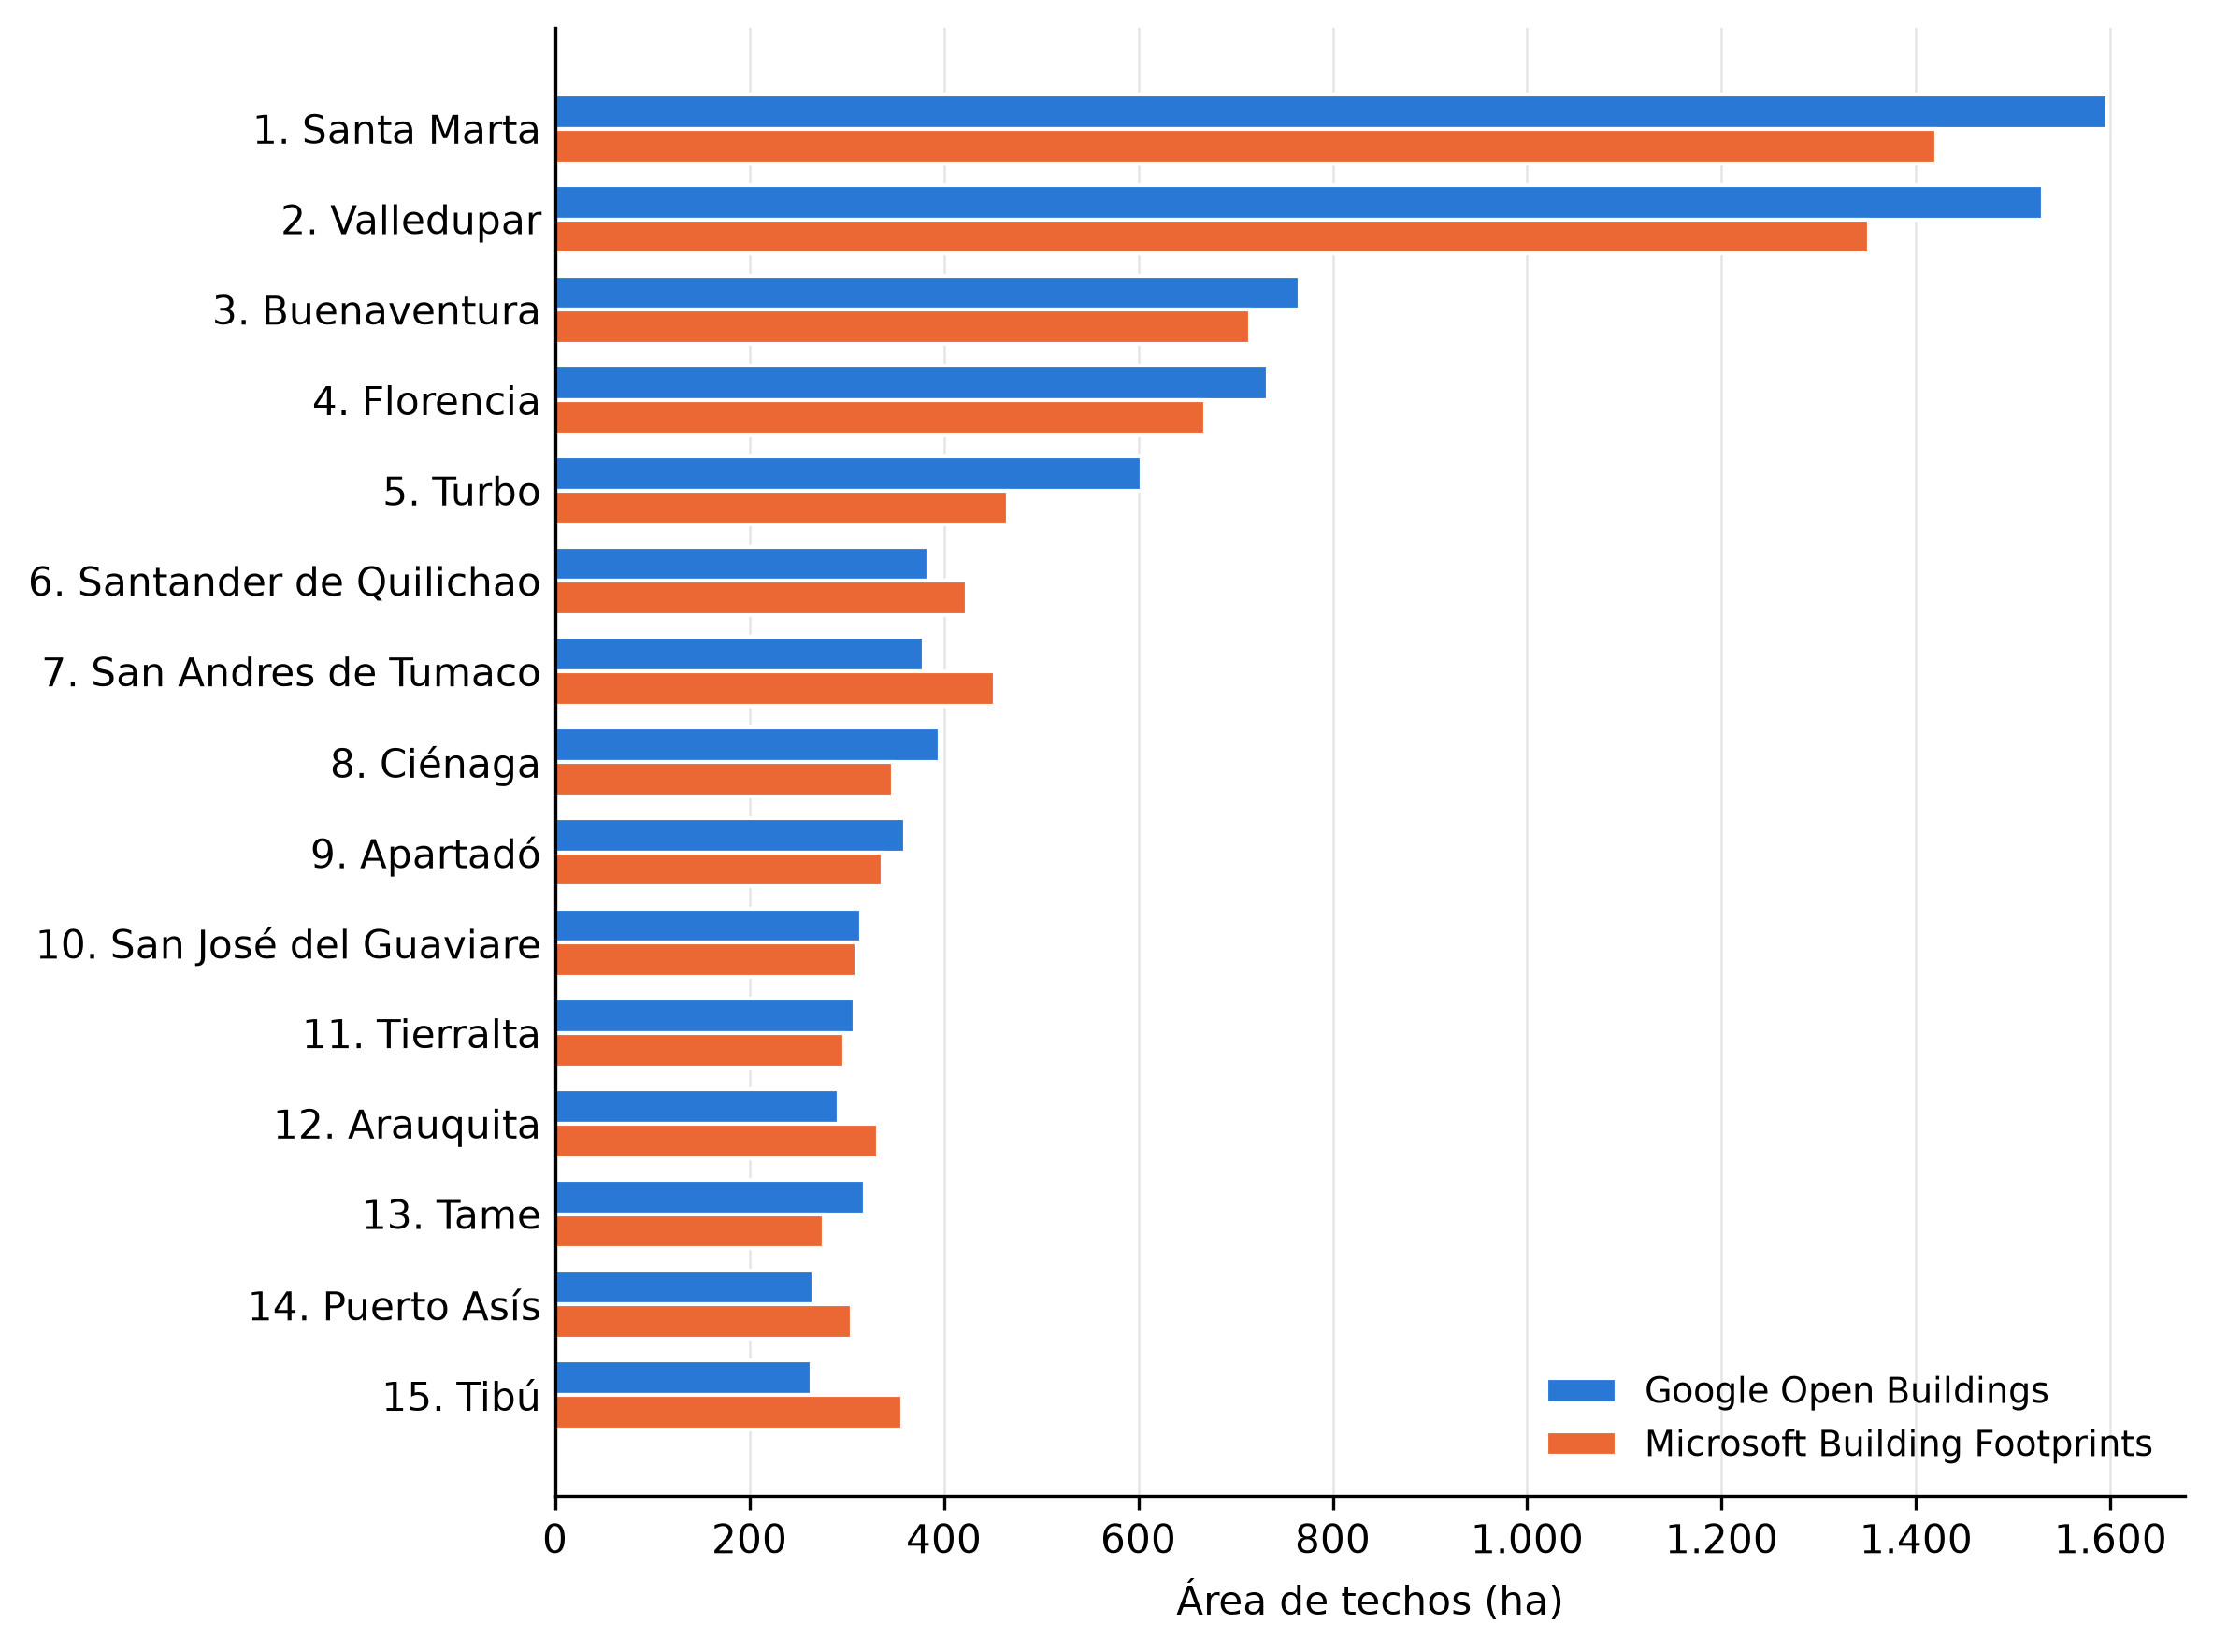
\includegraphics[width=0.95\textwidth]{img/ranking_top15.png}
  \caption{Área de techos de los 15 municipios candidatos según cada fuente,
  ordenados por el área conservadora.}
  \label{fig:ranking}
\end{figure}

\textbf{Lectura del ranking.} Los 15 municipios suman 7\,775\,ha de área
conservadora, el 39\,\% del total de los 170 municipios (20\,156\,ha), y
ninguno tiene las fuentes en desacuerdo: el criterio deja fuera, sin
necesidad de una regla adicional, a los municipios donde los datos no son
confiables. El ranking es estable: 13 de los 15 coinciden con el top 15 que
saldría de usar solo Google o solo Microsoft, y la sensibilidad al umbral de
confianza (tabla~\ref{tab:sensibilidad}) no cambia cuáles municipios lo
encabezan. Están representadas 11 de las 16 subregiones, con Santa Marta,
Valledupar y Ciénaga (Sierra Nevada - Perijá) a la cabeza.

\textbf{Por qué difieren las fuentes.} Se ven tres causas en los datos:
\begin{itemize}
  \item \emph{Tamaño de las huellas.} Google tiene 1,53 veces más edificios pero
        casi la misma área total, porque divide la misma superficie en huellas
        más pequeñas (82\,m\textsuperscript{2} de media frente a
        126\,m\textsuperscript{2} en Microsoft). Por eso el conteo de
        edificios no sirve para comparar fuentes y el ranking usa área.
  \item \emph{Huecos de detección en el Pacífico.} En el Chocó y la costa
        nariñense Google detecta muy poco o nada; una causa probable es la nubosidad casi
        permanente de la región, que reduce las imágenes útiles para el modelo. Es la
        zona donde se concentran 18 de los 23 municipios en desacuerdo.
  \item \emph{Fechas y modelos distintos.} Microsoft usa imágenes de 2014 a 2021
        y Google su propio modelo y periodo; una cabecera que creció en esos
        años tiene más área en la fuente más reciente, y cada modelo recorta
        de forma distinta los techos contiguos.
\end{itemize}

\textbf{Recomendación preliminar.} Para un piloto conviene empezar por los
municipios del top 15 que además tienen un porcentaje de techos alto, porque
el área está concentrada en un casco urbano y no dispersa en veredas:
Santa Marta, Santander de Quilichao y Apartadó están en el top 15 y entre
los cuatro municipios con mayor porcentaje de techos. Los municipios del Chocó y del Pacífico no deberían descartarse
por su área baja: ahí el resultado depende de la fuente más que del municipio,
y requieren verificación con imágenes o en campo antes de decidir.

% =====================================================================
% 10. Reproducción (Maria Camila)
% =====================================================================
\section{Reproducción paso a paso y entorno}
\label{sec:reproduccion}

\campo{src/analisis/run.py} encadena los pasos de la semana en orden y es lo
que corre \campo{make analisis}. Cada paso se ejecuta como
\campo{python -m src.analisis.<paso>}, igual que a mano; si uno falla, el
flujo se detiene ahí e indica cómo retomarlo con \campo{--desde <paso>}. Al
final imprime cuánto tardó cada paso.

\begin{table}[H]
  \centering\small
  \caption{Pasos de \campo{make analisis}, en orden.}
  \label{tab:pasos}
  \begin{tabularx}{\textwidth}{@{}l l L@{}}
    \toprule
    \textbf{Paso} & \textbf{Responsable} & \textbf{Qué produce} \\
    \midrule
    \campo{asignacion} & Jorge & \campo{cod\_mpio} en los edificios; registro en \campo{bitacora\_cargas} \\
    \campo{evidencia} & Jorge & \campo{explain()} con IXSCAN y con COLLSCAN \\
    \campo{validacion} & Jorge & Comparación con GeoPandas en 10 municipios \\
    \campo{agregacion} & Samuel & \campo{resultados}: 170 documentos por fuente y umbral, verificados \\
    \campo{sensibilidad} & Samuel & Tabla de sensibilidad al umbral de Google \\
    \campo{exportar} & Samuel & CSV por municipio y subregión; tabla por subregión \\
    \campo{figuras\_eda} & Jose Eduardo & Las cuatro figuras del EDA rehechas \\
    \campo{graficas} & Jose Eduardo & Dispersión por municipio y gráfica de sensibilidad \\
    \campo{mapas} & Maria Camila & Mapas por fuente, de diferencia y de \% de techos \\
    \campo{ranking} & Maria Camila & Top 15, tabla y gráfica; ranking completo en CSV \\
    \bottomrule
  \end{tabularx}
\end{table}

El flujo completo, desde una base vacía y sin datos descargados, es:

\begin{lstlisting}
git clone https://github.com/SamuOsorio/Proyecto-DBA.git && cd Proyecto-DBA
cp .env.example .env
python3 -m venv .venv && source .venv/bin/activate
pip install -r requirements.txt
# copiar el ZIP del MGN 2025 (nivel municipio) en data/raw/mgn_2025/
make all        # = make up municipios edificios analisis
\end{lstlisting}

Los parámetros no están escritos en el código: el umbral base y los umbrales
de sensibilidad, la regla de asignación, los CRS y las rutas de salida se leen
de \campo{config.yaml}, y cada documento de \campo{resultados} guarda en
\campo{parametros} el umbral, la regla, el CRS de las áreas y el commit del
código que lo produjo. Entorno: MongoDB 8 en Docker, Python 3.12 y las
versiones fijadas en \campo{requirements.txt}.

\figopcional{cap_make_all}{Corrida de \campo{make all} desde una base vacía:
resumen de tiempos por paso.}{fig:make-all}

% =====================================================================
% 11. Conclusiones (todos)
% =====================================================================
\section{Conclusiones, limitaciones y próximos pasos}
\label{sec:conclusiones}

El flujo quedó completo y reproducible: de los límites del MGN y las huellas de
dos fuentes abiertas hasta una colección \campo{resultados} con 170 documentos
por fuente y umbral, verificados contra los conteos de las colecciones, y
tablas, mapas y ranking que salen de la misma corrida. La asignación por
centroide usa el índice \campo{2dsphere} y coincide al 100\,\% con una
implementación independiente en GeoPandas en la muestra validada.

Las dos fuentes coinciden en el total (222 y 221\,km\textsuperscript{2}) y en
el orden de los municipios, pero no en el Pacífico, donde Google tiene huecos
de detección. Por eso el ranking usa el área que respaldan las dos, y ninguno de
los 15 municipios candidatos tiene fuentes en desacuerdo.

\textbf{Limitaciones.}
\begin{itemize}
  \item El área es la huella en planta: es un límite superior del área útil
        para paneles, porque no descuenta sombras, inclinación, orientación,
        tanques, ni techos que no soportan la carga.
  \item Las huellas vienen de modelos de aprendizaje automático sobre imágenes
        de fechas distintas; no son un catastro y tienen errores de omisión y
        de partición de techos.
  \item El área de techos no es potencial energético: falta cruzarla con la
        irradiación solar y la demanda de cada municipio.
  \item Un centroide justo sobre un límite puede caer fuera por la diferencia
        entre aristas esféricas y planas (un edificio de 4,5 millones).
\end{itemize}

\textbf{Para el informe final (26 de noviembre).} Integrar las cuatro entregas
en un documento autocontenido para la UPME; agregar una estimación de potencia
instalable con un factor de aprovechamiento del techo y la irradiación por
municipio; y proponer la verificación de los municipios del Pacífico antes de
descartarlos.

\end{document}
